\chapter{Method and materials}


\section{Study area} % flyttet først etter AMkomm
%mogleg å kjøre ein fin overgang fra intro til study area? Study area valt pga dårlige snøforhold i nyere tid -> vanskelig å gjere spor-tellinger -> denne delen av landet har starta med CT (\cite{Odden2015})


The mean annual temperatures ranges from 2-6 \celsius \ and precipitation lies between 700-1500mm (\cite{Moen1999}). 
Topography is predominantly flat towards the south, and more rugged and elevated towards the north. The landscape is a mosaic of forest and agricultural areas, divided with a wide network of gravel roads.
The area is situated in the southern boreal and the boreonemoral zones. %Må finne oppdaterte data (frå Norges vassdrags- og energidirektorat, 2019?)
Norway spruce (\textit{Picea abies}) and Scots pine (\textit{Pinus sylvestris}) make up the dominating boreal coniferous forests, with frequent presence of silver birch (\textit{Betula pendula}) and downy birch (\textit{Betula pubescens}), then aspen (\textit{Populous tremula}), alder (\textit{Alnus incana}) and black alder (\textit{Alnus glutinosa}).


%https://klimaservicesenter.no/faces/desktop/article.xhtml?uri=klimaservicesenteret/klimaprofiler/klimaprofil-oslo-og-akershus
%https://klimaservicesenter.no/faces/desktop/article.xhtml?uri=klimaservicesenteret%2Fklimaprofiler%2Fklimaprofil-buskerud  
The study area (59.36-60.45° N, 9.31-11.13° E) extends over much of the southeastern parts of Norway in municipalities Flå, Krødsherad, Sigdal, Ringerike, Modum, Hole, Lier, Øvre Eiker, Asker, Oslo, Enebakk, Indre Østfold, Våler, Råde, Moss, Frogn and Vestby in Oslo and Viken counties. 
The climate has a continental character due to rain shadows of the mountain ridges from the west. 


Growing season length was 170 - 190 days (Moen 1999) % |AMkomm: fjern map 6, s.21, men sett hvor det er rent geografisk 


\section{Study species} %Usikker på om eg skal ha med
%\subsubsection{Rev}  ?

%We also collated information on average body and home range sizes for a subset of species surveyed in the reviewed studies in order to better quantify the functional diversity of wildlife being sampled by CTs and to evaluate the degree to which CT methodologies were tailored to focal species. Burton 2015

The species I'll focus on in this thesis are the species that most frequently was observed \emph{(>50 events)}, excluding farmed animals (e.g. cattle), humans and dogs, and grouped categories of animals (e.g. birds).
%Although decisions on camera placement (height and angle) were made with the aim on photo capturing lynx, I have also included smaller species in the analysis.

% Idea sprung from reading Meek 2014 guiding principles; Height of camera and, distance to centre of detection zone or lure.
%Growing skeptical to the validity of my argument now that I know about the random effect in models. As I argued in my own notes when reading the Meek article I don't think I need to "take these biases into consideration" because I'm trying to detect differences between the same cameras.

%This includes three species, . 


The species I have included in my analyses are roe deer (\textit{Capreolus capreolus}), red fox (\textit{Vulpes vulpes}), badger (\textit{Meles meles}), moose (\textit{Alces alces}), red deer (\textit{Cervus elaphus}), red squirrel (\textit{Sqiurus vulgaris}), hare (\textit{Lepus timidus}), European pine marten (\textit{Martes martes}) and lynx. 




\section{Study design} 
The Norwegian Institute of Nature Research (NINA) started with CTs to substitute snow track surveys of lynx family groups, after several years of varying snow season length in south eastern Norway (\cite{Odden2015}). The surveys are integrated in a coordinated Scandinavian science project on lynx, called Scandlynx. 

I was given access to CTs used in the Scandlynx project, and chose the 60 % |AMkomm: Fra hvor mange og hvorfor? 
sites closest to Oslo (for logistical reasons) which weren't already equipped with white LED light. 
Instead, these were equipped with either black or IR flash, but I will refer to them as the IR CTs. 

The IR CTs had been installed on trees 1-3 m from wildlife, human or tractor paths, 30-160 cm above ground level, and their distance from houses or roads varied to a large extent.
They were set up and handled by people from NINA and, at the sites further from Oslo, by local volunteers. %members of the Norwegian Hunters and Fishers Society (NJFF). 
The installation of the cameras did not follow a strict protocol, nor were their locations chosen randomly. The overall placement was systematic as decided by NINA, then there was a deliberately-biased placement of the CTs put up in areas where the individual handler deemed it most likely to photograph lynx, and hence, based on a combination of site accessibility and expectations of animal occurrence. % slik som (\cite{Burton2015} seier skal formidlast). 

%\emph{presence of natural or artificial attractants may draw animals in to a CT} \cite{Burton2015}.

\begin{figure}
    \begin{center}
    	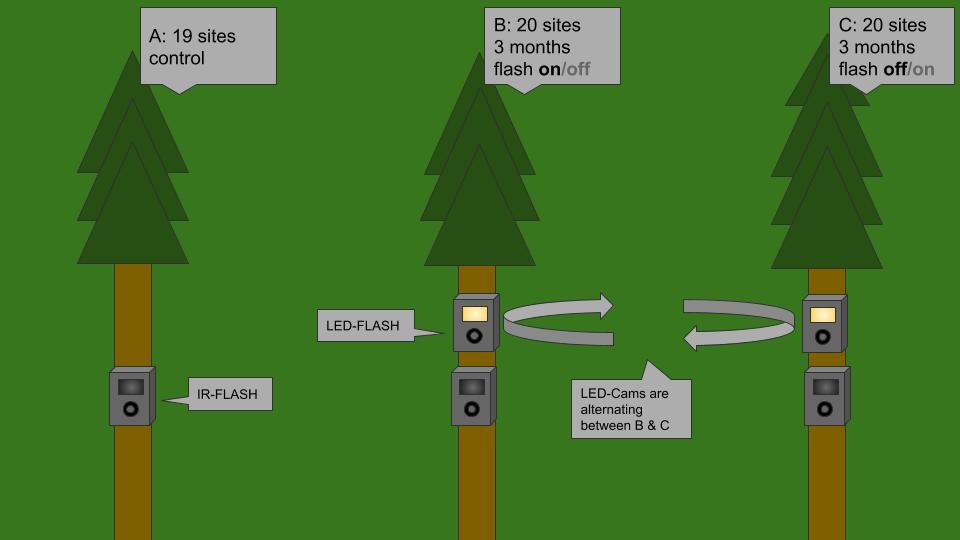
\includegraphics[scale=0.5]{./img/experiment_setup.jpg} %insert figure of groups     
    \end{center}
\caption[Experiment setup]%
    	{Experiment setup \par \small I chose 60 sites with preinstalled Infrared Camera Traps (IR CTs) for my study, and divided them into three groups, where the first group remained unchanged (control group), and the two other alternated on having additional white LED CTs present (treatment groups). Four sites were removed from the analysis due to large gaps in the data, etc.}
    \label{fig:exp_set}
\end{figure} 


I divided the sites randomly into three groups of 20 sites. Cameras in the first group remained unchanged as a control.
The remaining two groups (hereby referred to as treatment groups) were equipped with an additional white LED camera (Reconyx PC850; hereby referred to as the LED CTs) in alternating 3 month-periods, as illustrated in figure\vref{fig:exp_set}.


%After approximately three months, I moved the LED CTs to the other treatment group. The periods were marked as LED\_1, LED\_2 for first and second LED period, and IR\_1, IR\_2 for first and second IR period as seen in figure \vref{fig:timeseries}.
I set up all LED CTs above the IR CTs already in place (installation examples in figure \ref{fig:cam_ex_main}). 
At one site the IR camera had been installed so far above ground level that I chose to position the LED CT below the IR CT. %Atle fjerna kryssref til bildet

The camera boxes containing the LED CTs remained at each site untill the end of the experiment. Note that the second treatment group had no extra boxes before the start of their first LED period in May 2019 (i.e. remained identical to the control group untill May).   




\begin{figure}
		\begin{subfigure}{.5\textwidth}
		  \centering
		  	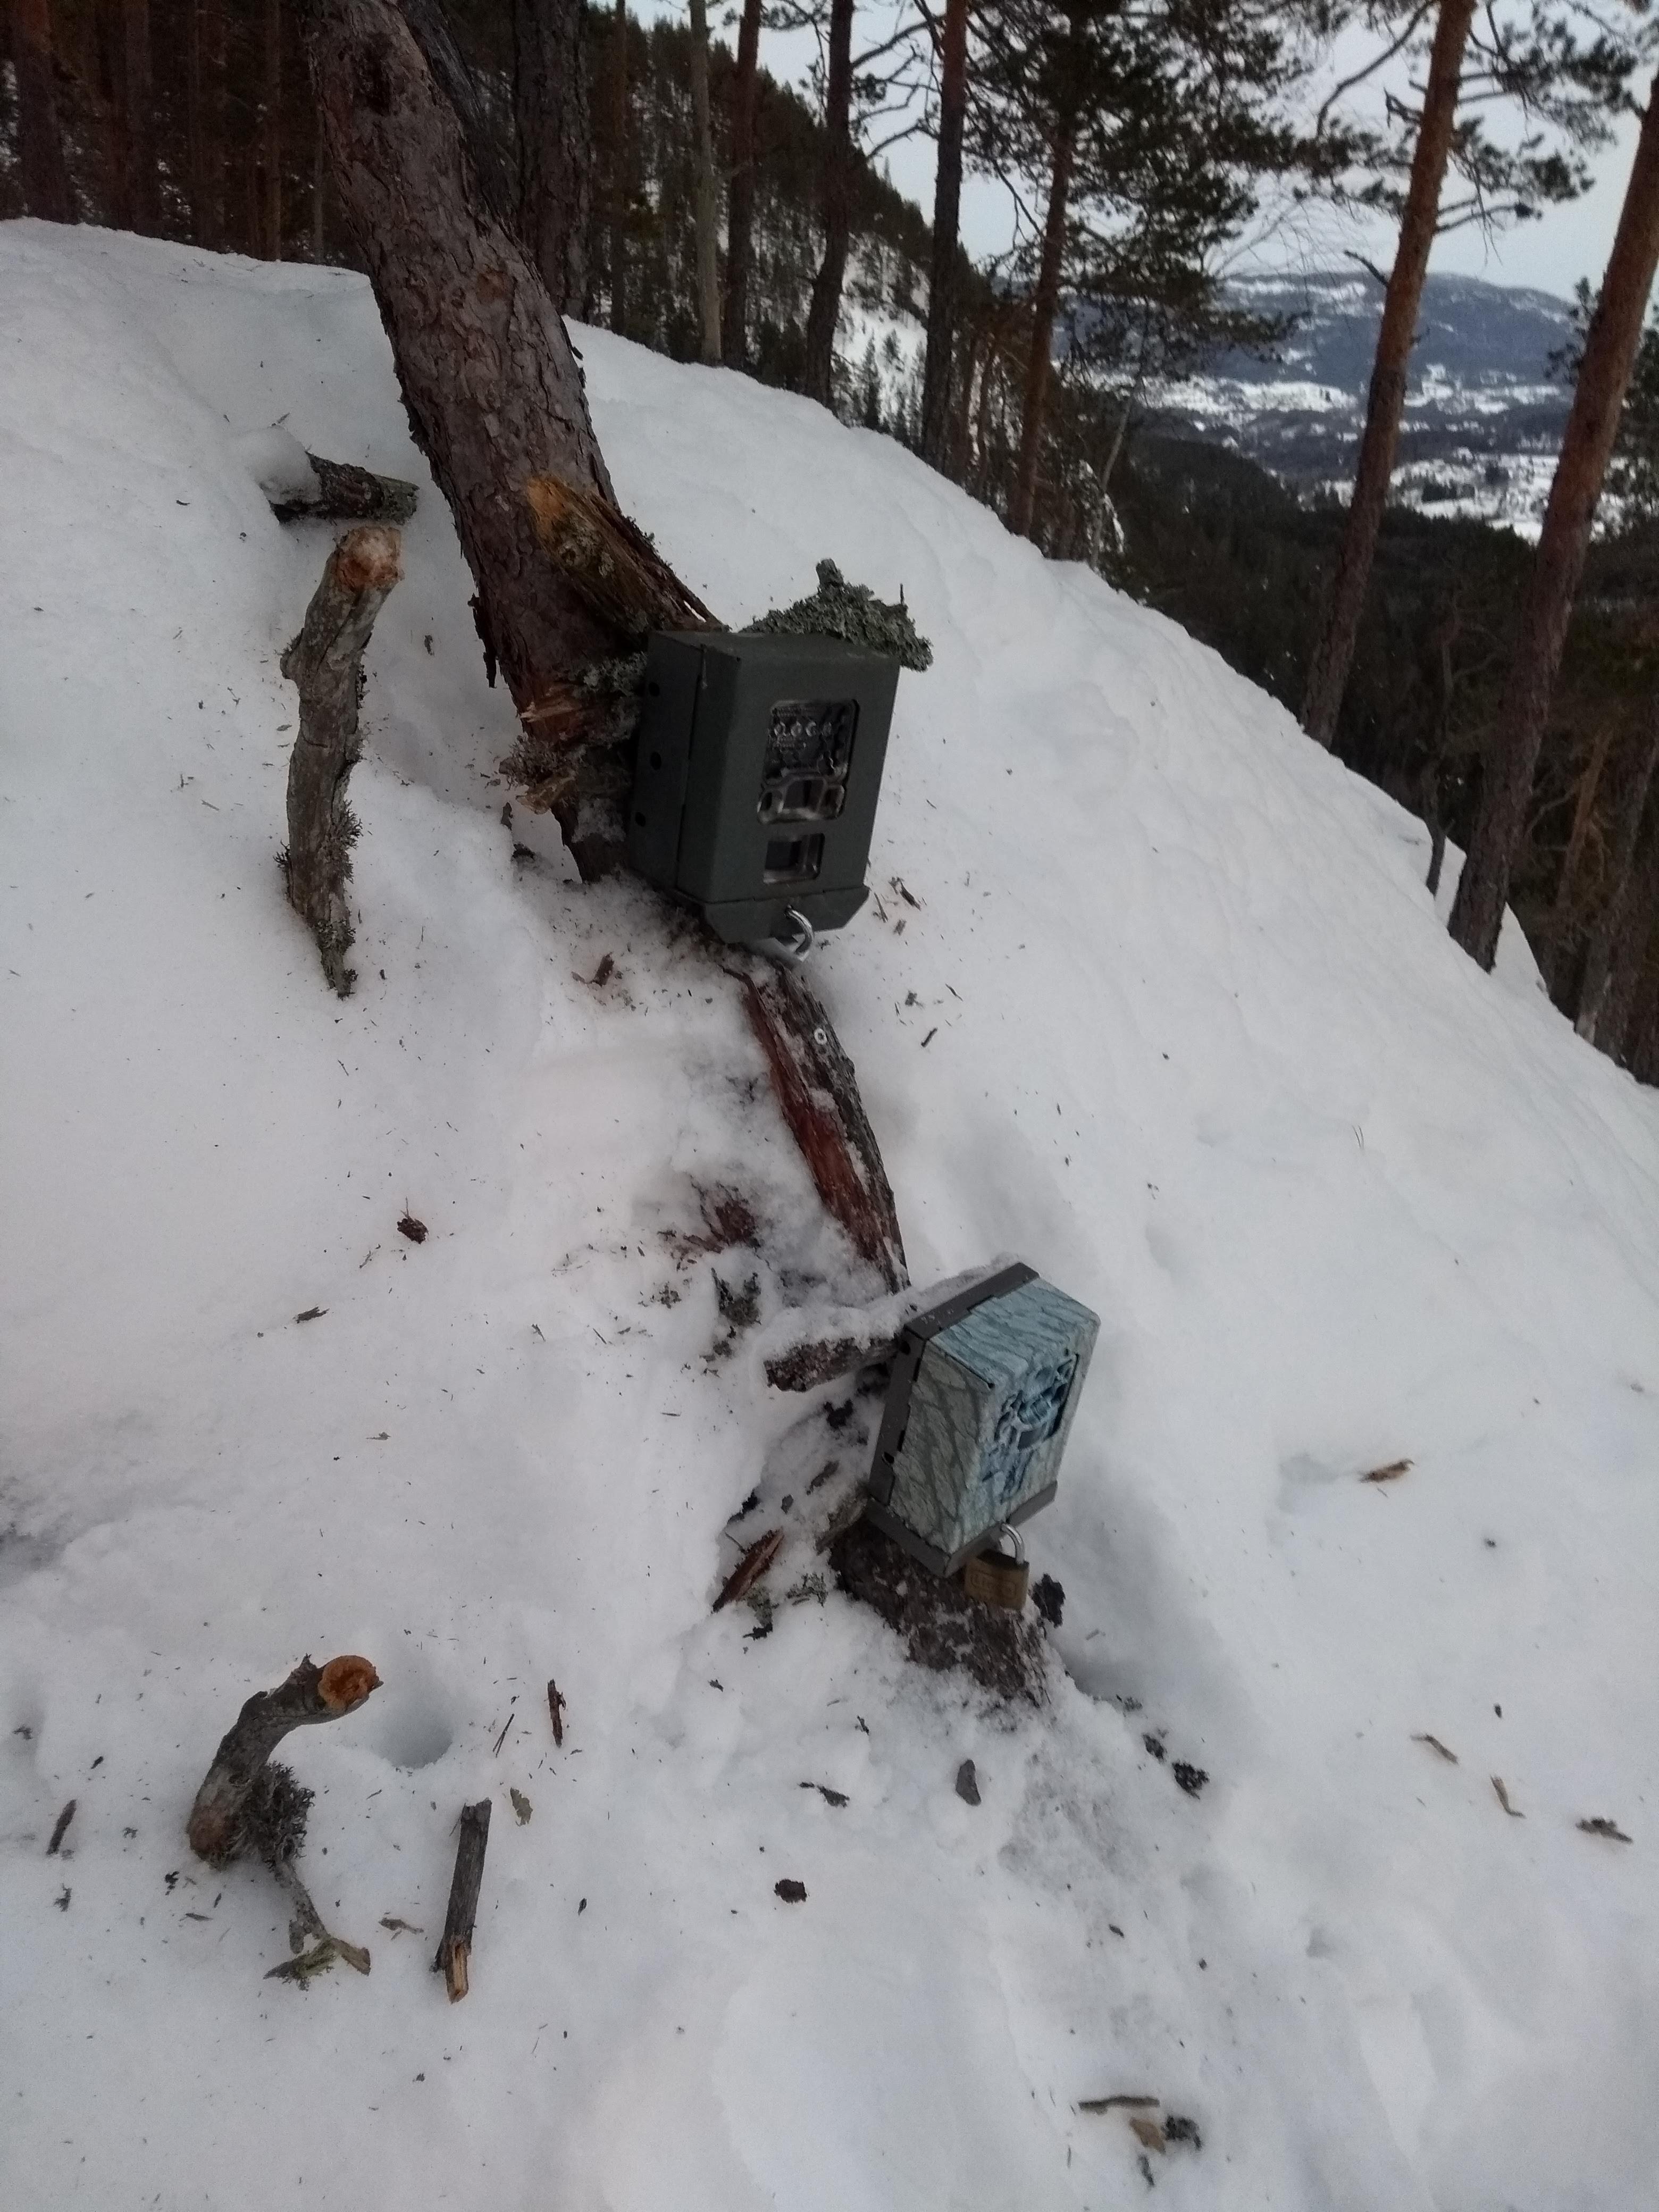
\includegraphics[width=.8\linewidth]{./img/cam_install_example/IMG_20190212_161615169.jpg}
		  \caption{Browning IR installed on fallen tree.}
		  	\label{fig:cam_ex_a}
	\end{subfigure}
		\begin{subfigure}{.5\textwidth}
		  \centering
		  	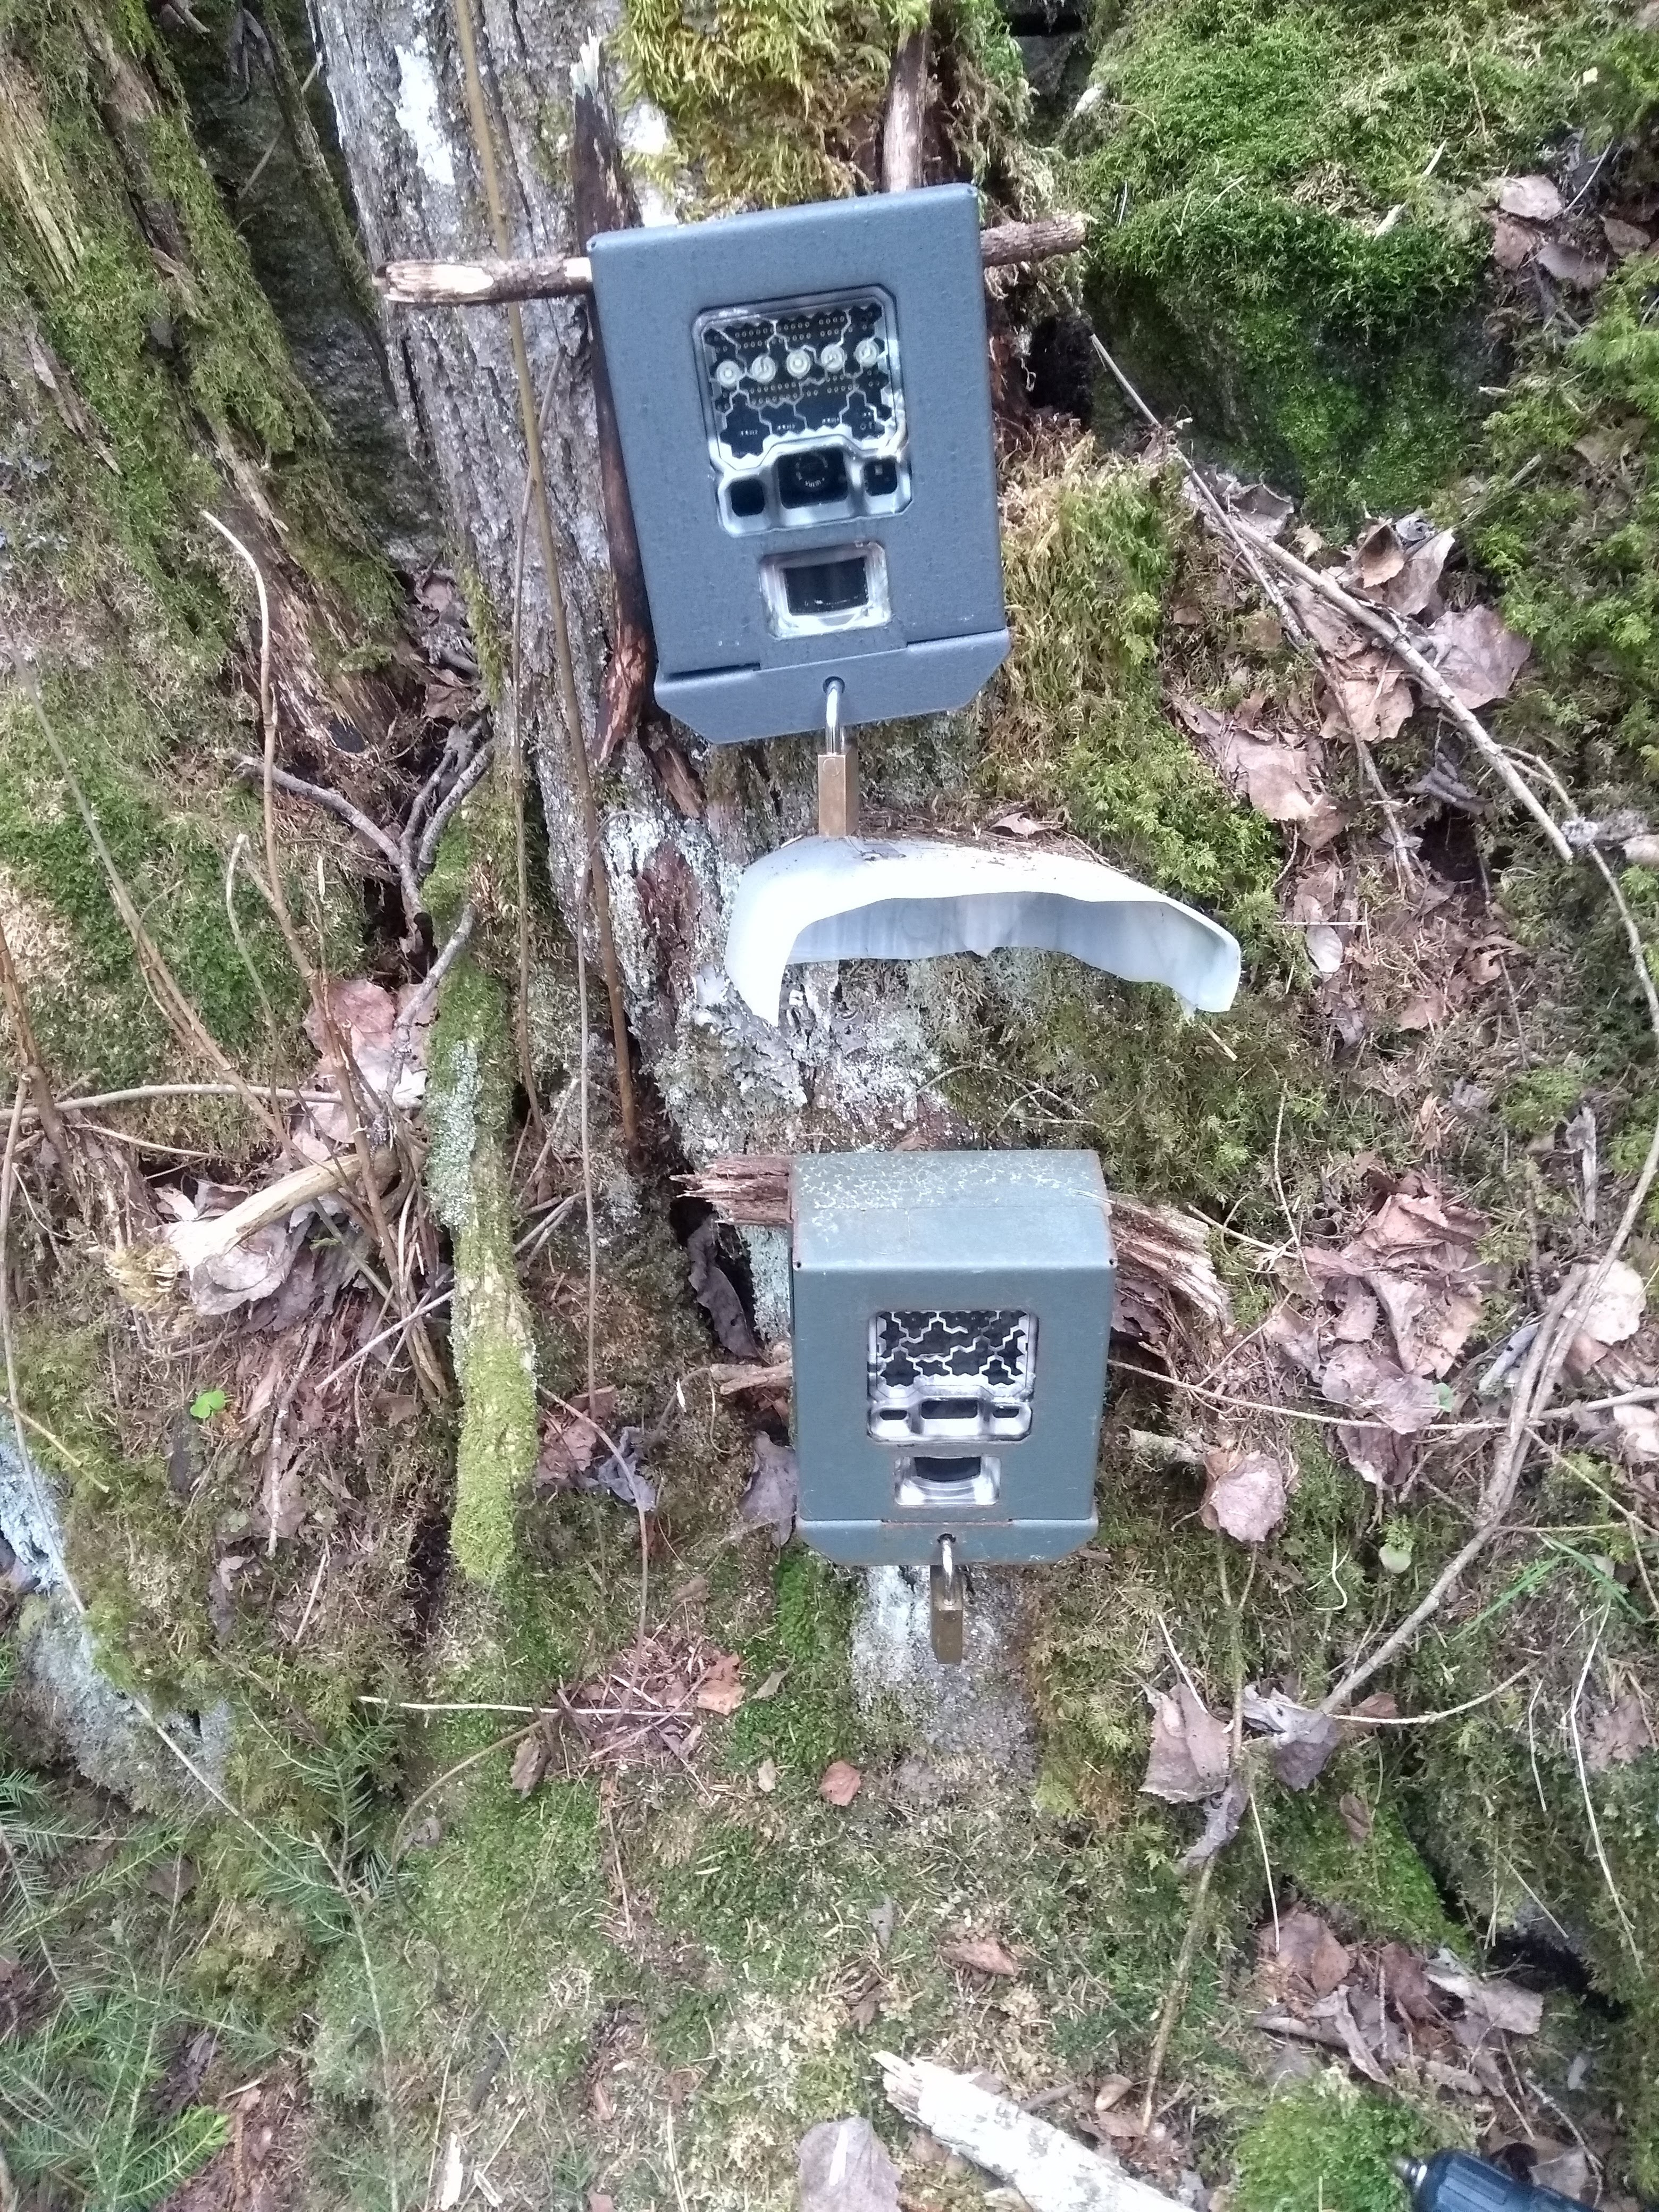
\includegraphics[width=.8\linewidth]{./img/cam_install_example/IMG_20190515_170952923.jpg}
		  \caption{Reconyx IR installed with snow cap.}
		  	\label{fig:cam_ex_b}
	\end{subfigure}
		\begin{subfigure}{.5\textwidth}
		  \centering
		  	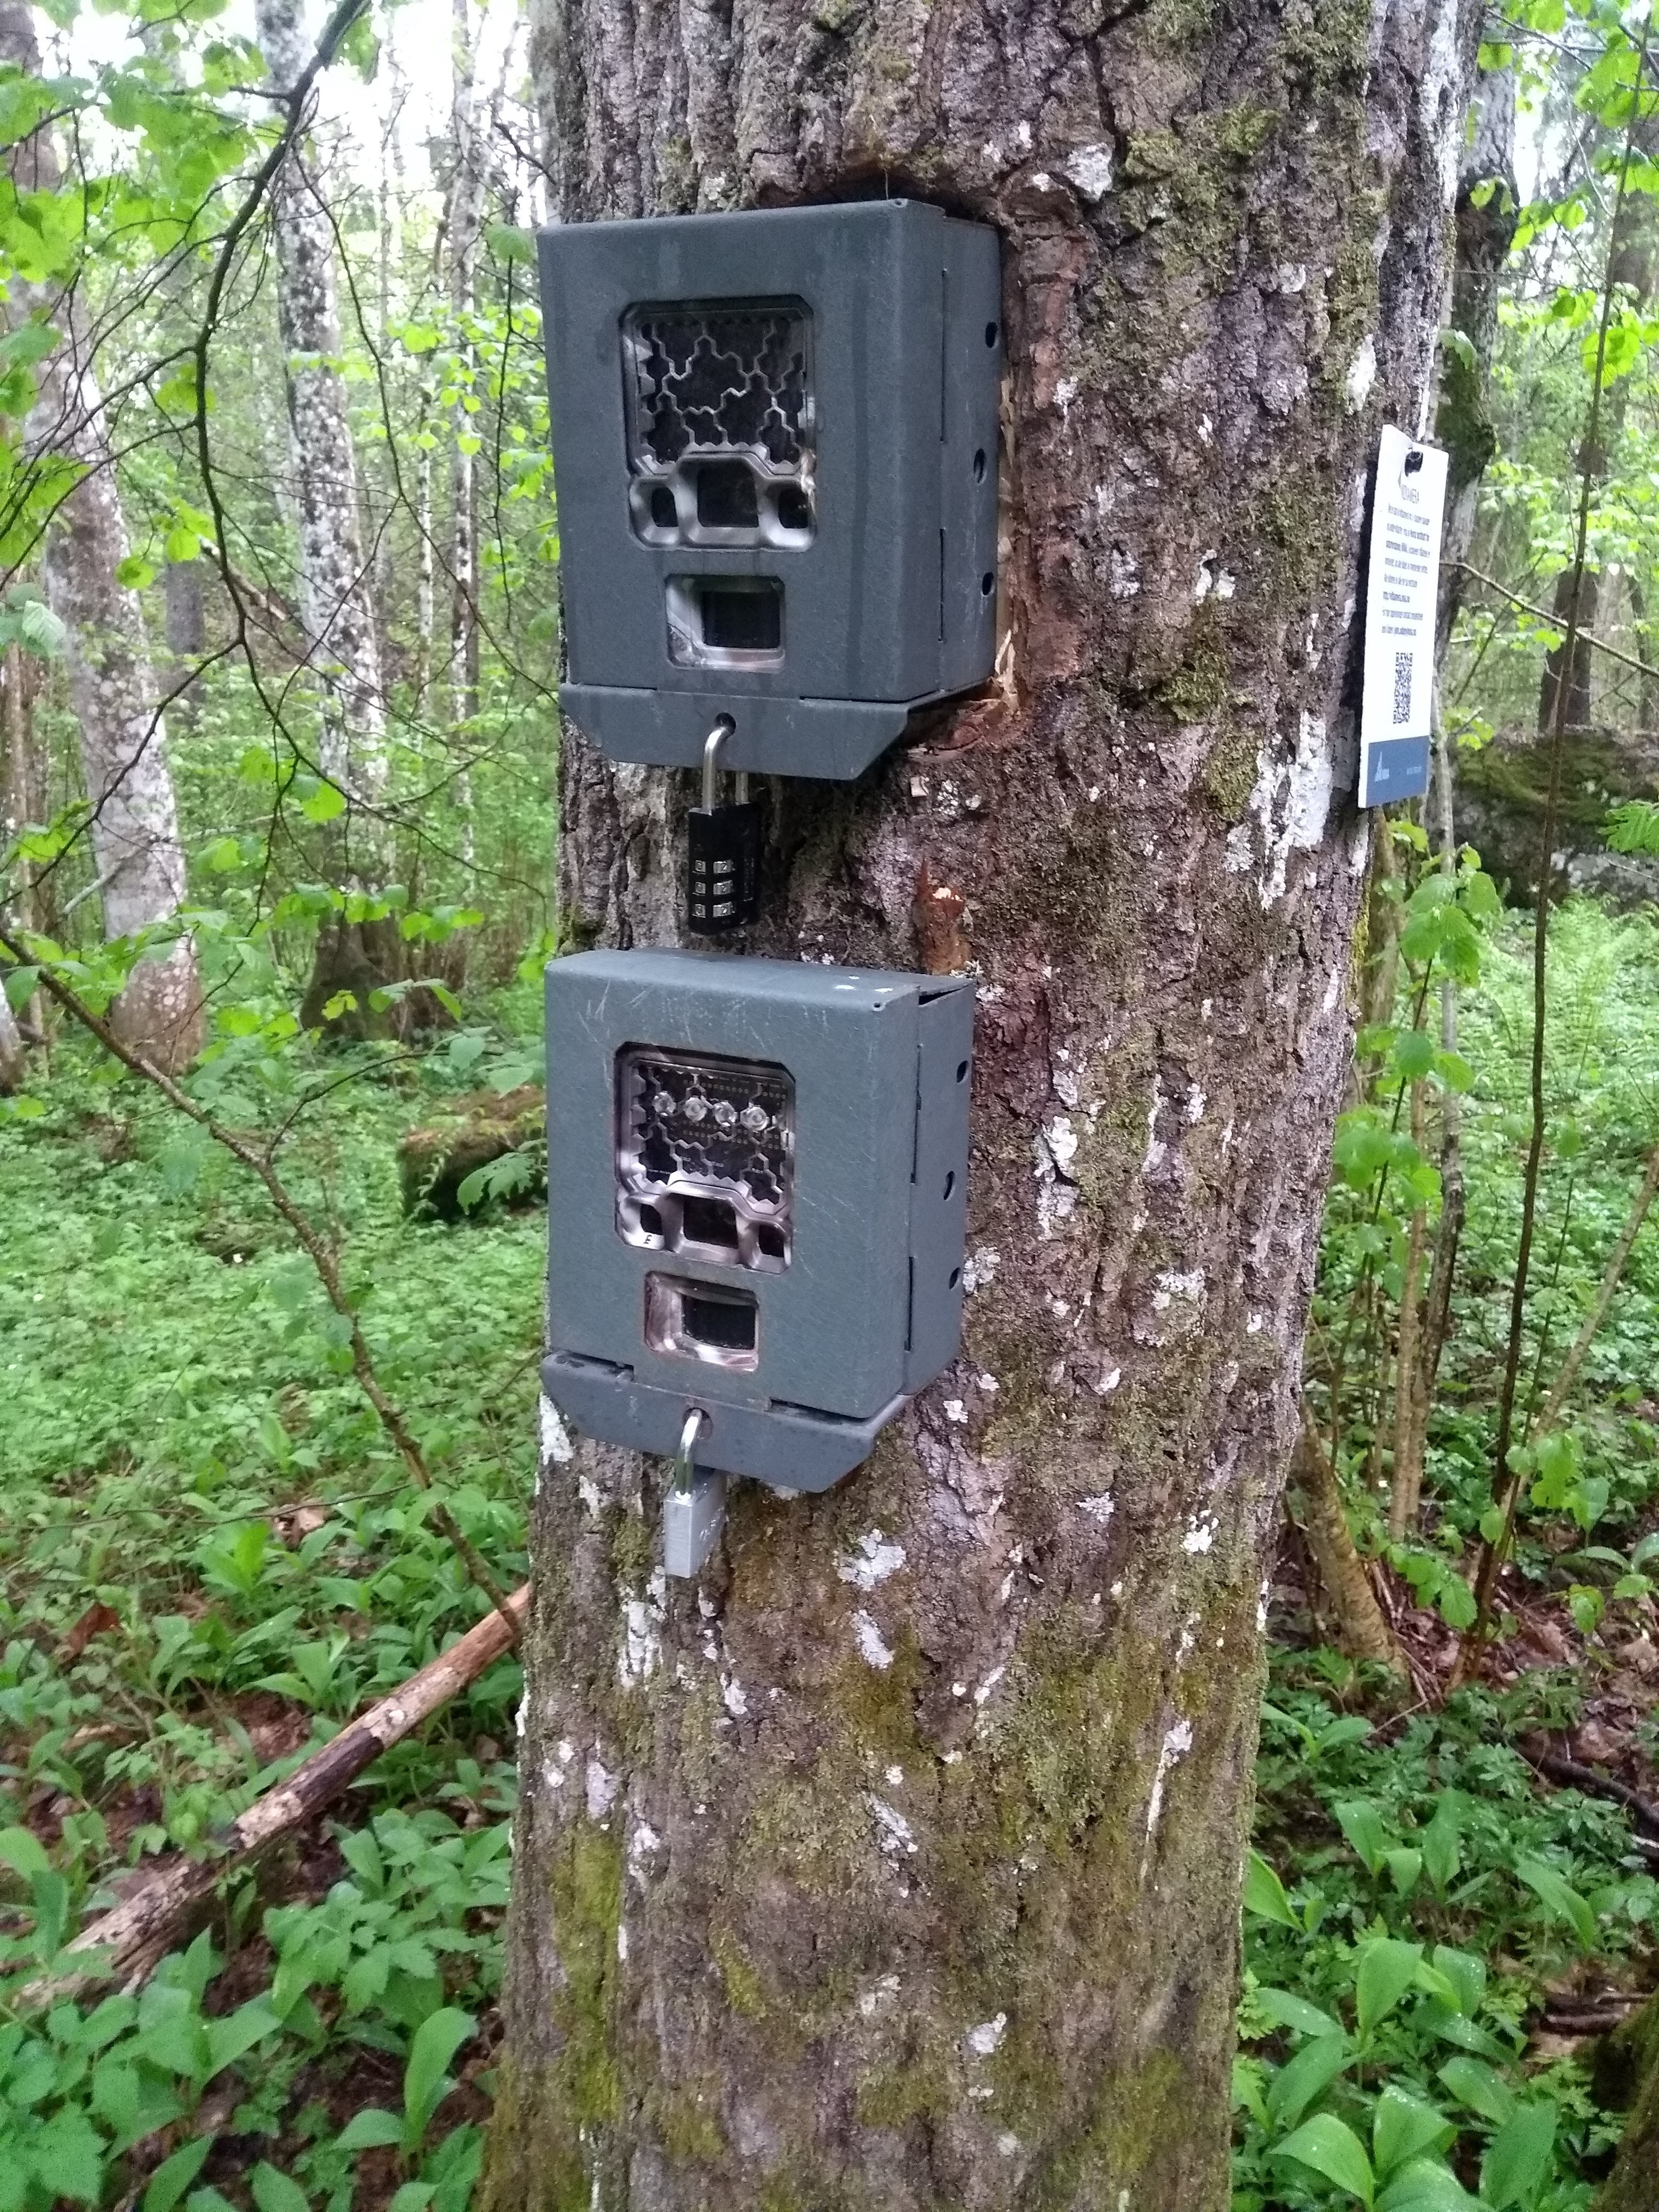
\includegraphics[width=.8\linewidth]{./img/cam_install_example/IMG_20190521_181329313.jpg}
		  \caption{Reconyx IR 160 cm above the ground.\\ Therefore, I positioned the wLED underneath.}
		  	\label{fig:cam_ex_c}
	\end{subfigure}
		\begin{subfigure}{.5\textwidth}
		  \centering
		  	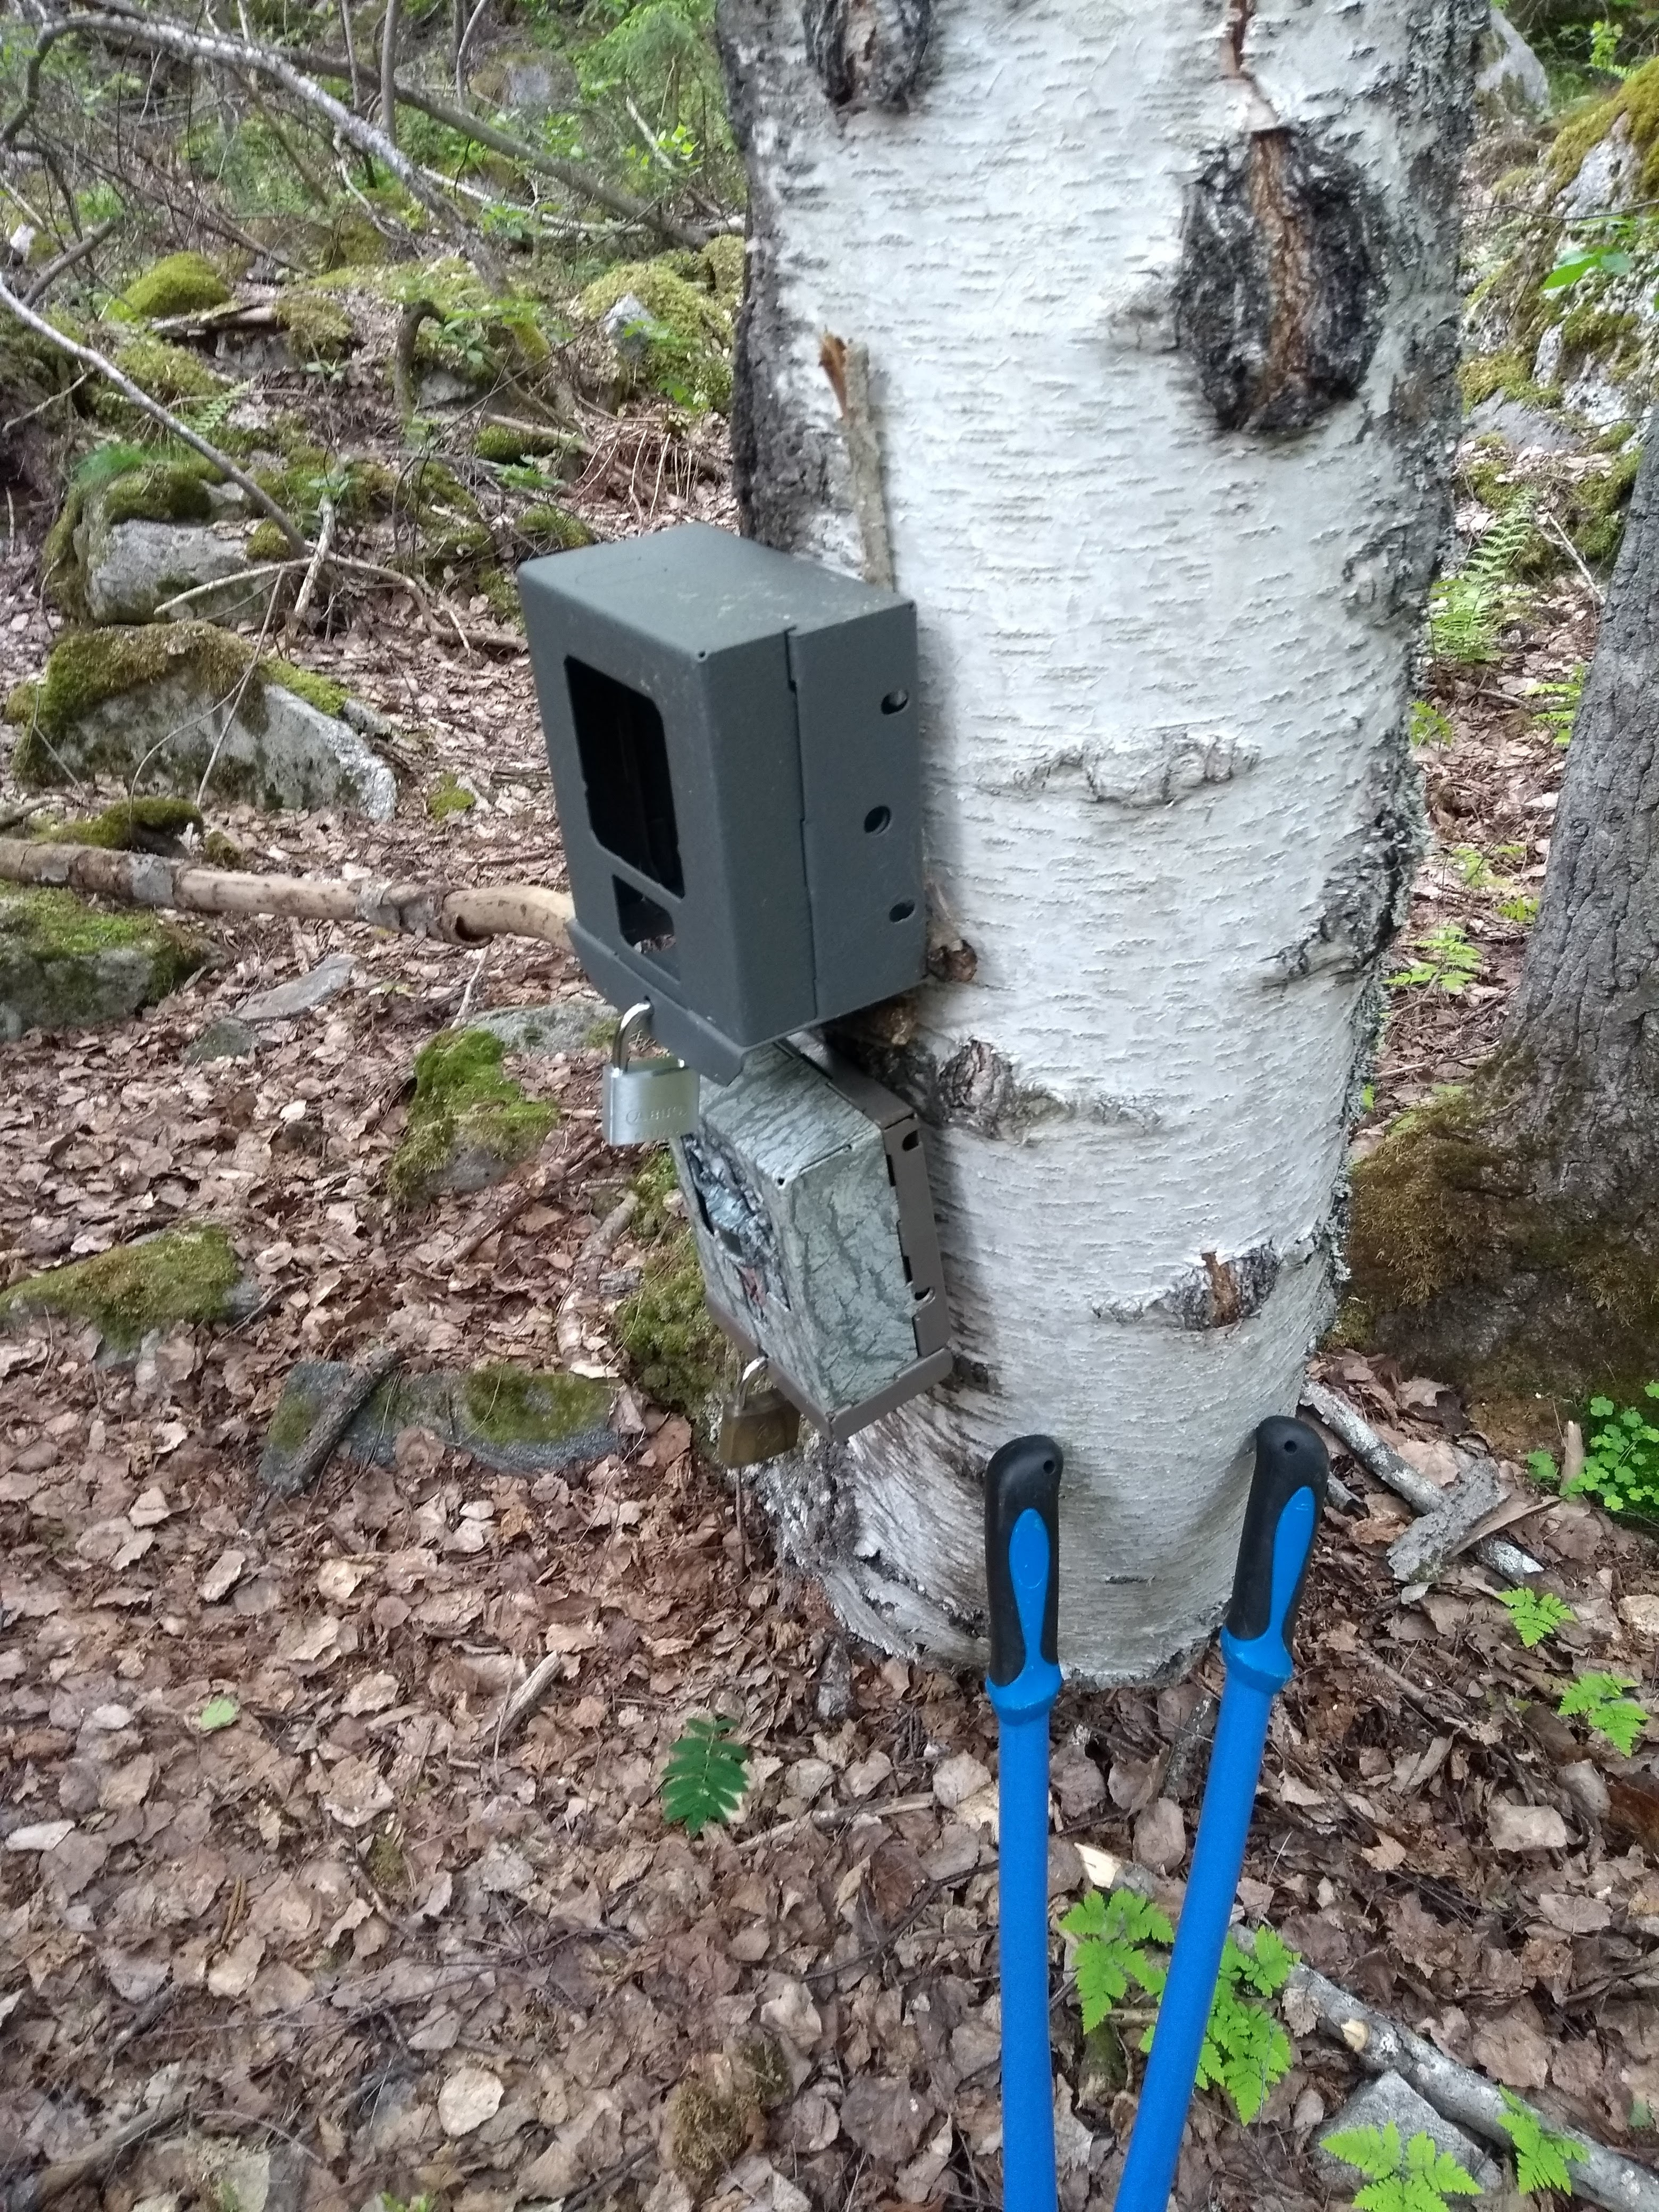
\includegraphics[width=.8\linewidth]{./img/cam_install_example/IMG_20190529_181049340.jpg}
		  \caption{Additional CT boxes remained\\ during IR periods.}
		  	\label{fig:cam_ex_d}
	\end{subfigure}
		\caption[Examples of camera setups]
		{Examples of camera setups %\par \small
		The preinstalled IR cameras varied in the way they were set up. Lower cameras had Infra-Red flash, upper cameras had white LED flash.}
	\label{fig:cam_ex_main}
\end{figure}





I visited sites of the treatment groups at least once every three months in order to move the LED cameras.
For logistical reasons I visited sites of the control group less often.
However, as the cameras were part of other, ongoing projects, they were occasionally visited by workers from NINA to retreive the Secure Digital memory cards (hereby SD Cards) for data. %write in full on first mention (-Atle)
This was mostly the case for sites close to, and south of, Oslo, or rather, the cameras not normally operated by members of the NJFF.

When doing the analyses I needed periods of similar lengths to each other. Therefore, I divided the control group-cameras into four periods of similar lengths to that of the treatment group cameras (see figure \ref{fig:timeseries}). %TODO flytte til analyse-del?


%We quantified the degree of consistency in implementing and reporting features of CT protocols and study design that might affect detectability and sampling error (e.g. camera type and settings, spatial and temporal sampling effort, use of attractants; Table S1). These details are fundamental to interpreting results of CT studies and assessing their reliability, repeatability and suitability for broader comparison or synthesis (Meek et al. 2014a)

%TODO Details of camera trap orientation, use of lures, and performance settings are also critical elements of camera trapping methodology. The height in relation to the target, the direction the camera is facing in relation to expected animal travel and path of the sun as well as horizontal and vertical alignment may all influence the results of camera trap studies. Providing clear descriptions of exactly how cameras were placed is fundamental to understanding and interpreting the results of research. (Meek etal 2014)

%!!! Her må eg også beskrive vegetasjon-fjerning, bruk av drill for å feste kameraboks, etc. %TODO

%Whenever I noticed vegetation blocking the view of the camera, or excessively triggering it, I removed the vegetation.



\section{Data Collection} 
%The fieldwork was conducted between September 15 and December 20, 2017. In this study, camera traps from the Norwegian Institute for Nature Research (NINA) were used. NINA uses camera traps to monitor the Eurasian lynx in southeastern Norway as part of the SCANDLYNX project (Odden, 2015). SCANDLYNX is a Scandinavian research project on the Eurasian lynx (Odden, 2015; SCANDLYNX, 2017). Camera traps were placed specifically with the goal to photo-capture lynx, and were therefore placed in steep terrain, on ledges or facing the cliff bases, often close to wildlife trails. The cameras were pointing perpendicular to the wildlife trail at locations where a wildlife trail was present. Each camera was mounted on a tree between 0.2 and 1 m above ground

Five different models of RECONYX™ (address: 3828 Creekside Ln, Ste 2, Holmen, WI 54636, USA, www.reconyx.com) cameras were used, 
and one model of BROWNING™ (address: One Browning Place, Morgan, UT 84050, USA, www.browningtrailcameras.com), details in table \ref{tab:cam_mod}.

Reconyx-cameras have been reported of having an average trigger speed of 0.2 seconds, whereas the Browning model was reported an average of 0.7 seconds (Trigger speed shootout, \cite{Trailcampro2014}).



\begin{table}[h]
\caption{Camera models included in the survey}
\label{tab:cam_mod}
\centering

\begin{tabular}{llr}
\hline
Producer  & Model name & Flash type  \\
\hline 
Browning	& Spec Ops: Extreme 					& No-glow IR \\
%\multirow{5}{2cm}{Reconyx HyperFire Series} &
			& HC500 Semi-Covert IR					& Red-glow IR \\
Reconyx		& HC600 High-Output Covert IR			& No-glow IR  \\
HyperFire 	& PC800 Professional Semi-Covert IR 	& Red-glow IR \\
Series 		& PC900 Professional Covert IR 			& No-glow IR  \\
    		& PC850 Professional White Flash LED	& White LED  \\
\hline
\end{tabular}
\end{table}


\begin{table}[h]
\caption[Camera settings and features]
{Camera settings and features %\par \small 
All Reconyx-models were part of the HyperFire series and practically identical in all aspects except for type of flash. Camera specifications are gathered from product reviews (www.trailcampro.com).}
\label{tab:cam_set}
\centering
\begin{tabular}{lcc}
\hline 
 & Browning & Reconyx \\ 
\hline 
Number of cameras 	& 34(?) 	& 26(?) \\  
Trigger speed 		& 0.43 s 	& 0.28 s \\ 
Recovery speed 		& 0.8 s 	& 0.9 s \\ 
Photos per trigger 	& 8 		& 3 \\  
Detection angle 	& 45.5$^{\circ}$ 	& 42$^{\circ}$ \\ 
Field of view 		& 40.6$^{\circ}$ 	& 42$^{\circ}$ \\  
Quiet period 		& No delay 	& No delay \\ 
Trigger interval	& Rapid fire & Rapid fire \\
Time lapse			& No	 	& Yes \\
\hline 
\end{tabular} 
\end{table}



%( CT model and settings (quiet period, SENSOR SENSITIVITY, trigger speed, photograph, burst of photographs or video, type of flash, etc.) ) %TODO add into cam_mod table




% [Detection shootout 2017](https://cdn.shopify.com/s/files/1/1065/8354/files/2017_Detection_Shootout_8de2600d-eb3a-42a8-9420-728aae5056e5.pdf?12422955367088316008)



Cameras were operating 24 hours per day. The RECONYX™ cameras were set to take one time lapse photo per day in order to verify that the cameras had been operational.
They were set to take 3 pictures per series, as fast as possible using \emph{rapidfire}, and retrigger immediately using \emph{no delay}.

The BROWNING™ cameras were also set to rapidfire, but to 8 photos per trigger, which unfortunately made the memory cards more vulnerable to filling up before being collected. This happened in some areas with sheep and/or cattle, and sometimes due to triggering by vegetation.

Therefore, the BROWNING™ cameras tended to have more gaps of inoperable days.
The true number of active camera days are confounded by the lack of time lapse photos from the BROWNING™ cameras. To approach the true number of active days, I assumed all Browning cameras to be functional every day, unless the camera was inactive when I visited it. In that case, I considered the camera inactive since the day of its last photo.


As seen in figure \ref{fig:map}, %TODO insert map with loc, white point inside flash-cameras.
there was a correlation between latitude and camera type.

% difference between the two camera types*** 
% Assumptions: chance of detection & sp validation BROWNING > RECONYX, operational days BROWNING < RECONYX


\begin{figure}
	\label{fig:map}
\end{figure}




\section{Data processing} %TODO
All SD cards were delivered to NINA for data processing.
Firstly, a facial recognition algorithm (FRA)  is used to sort all the pictures. %artificial intelligence software (AI)
Afterwards, a human sorter checks the softwares' output, confirming all the correct decisions (i.e. species detections) and correcting all the wrong ones. 
Consequently, the rate of correctly identified species has gone up as the FRA sometimes detect animals that aren't easily noticed by human sorters (pers.comm. John Odden). 
The goal is to fully automate this identification process, which is a request from The Norwegian Data Protection Authority (DPA) in relation to usage of cameras in densely crowded areas (e.g. parks).



%Nei, vi har ikke publisert artikkel på gjenkjenningsalgoritmen. Du har jo vært med på prosessen sjøl, så jeg veit ikke om du egentlig trenger referanse her, men du kan sette inn John O som pers med og merke det, så kan han eller jeg endre det slik vi mener det bør være når vi leser gjennom oppgava di..


The output I got as a result was a data frame containing a time stamp for every time the CTs were triggered, %kvar gong eit bilde blei tatt
including all meta data from the camera, coupled with predicted species (FRA output, with a confidence number), verified species (by human sorters), number of animals and distance from camera.

%Describing in brief how coding is undertaken is useful for readers to understand the methods used in relation to the results.(Meek etal 2014)


I defined one event as any one species passing with a buffer of 30 minutes untill next detection of the same species, %TODO  Må formulere betre
in order to remove autocorrelation in observations, e.g from ruminating individuals. 
Number of individuals and distance to CT were not taken into account. 


My predictor variable of interest was a three level factor, where LED represented the periods with an additional white LED CT present, IR represented the periods \emph{after} a white LED CT had been present, and Control represented all periods where a white LED CT had never been present. The different periods are visualised in figure \ref{fig:timeseries}. 


4 sites were removed before the analysis due to technical faults, etc. %TODO språkvask
1 CT from the control group, as it turned out to be a white LED camera.%present in tabular?
3 CTs from the treatment groups, because of large or frequent gaps due to technical errors, and ineffective placement of the additional white LED camera. 



\begin{figure}
		\centering
		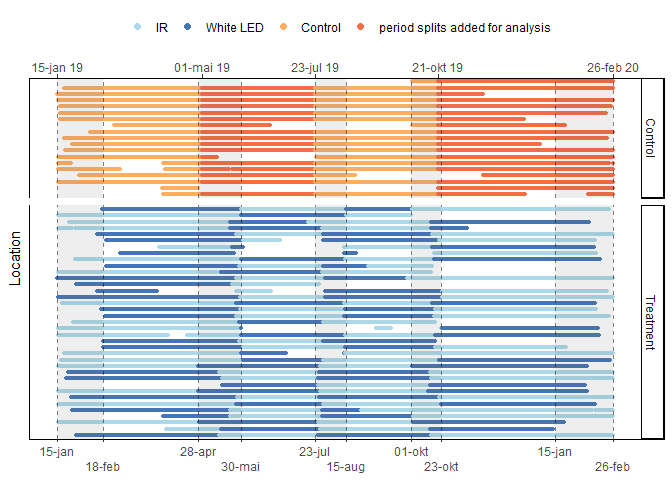
\includegraphics[scale=.8]{../R/FLM_notebook_files/figure-gfm/effort-facet-1.png}	
\caption[Active camera days]%
{Active camera days \par \small Colours indicate the different periods for each camera. White spaces indicate gaps where the IR CTs were inactive. Control camera periods were defined in similar lengths to that of the treatment group during analysis. As a result, "day 0" of Control-cameras are often set at dates far from an actual visitation day. Shaded areas represent my field work periods. The first IR period of the second treatment group was defined as "Control" for the analysis, as they remained unchanged untill their first LED period. \label{fig:timeseries}}
\end{figure}


%*************************************************************
%
%Hypothesis 1: Usage of white LED flash will stress one or more species in general, and therefore lower the detection rate of the stressed species. The effect will likely vary in extent between species.
%
%*************************************************************
%
%Hypothesis 2: The effect of the white LED will correlate with urbanisation-factors, as individuals that live closer to urban areas are habituated to Artificial Light At Night (ALAN), and thus will have a weaker response to the white LED
%
%


\section{Statistical analysis} %This is a reference to the session info appendix \ref{app:sessinfo}

To test for effects of the white LED flash I used the R programming language (\cite{RCoreTeam2020}), in the RStudio IDE (\cite{RStudioTeam2020a}), adopting large parts of the tidyverse (\cite{tidyverse}) and the easystats (\cite{easystats}) frameworks along the way. Complete citation of R packages used are presented in appendix \ref{app:sessinfo}. %Atle: Why sessioninfo?
%TODO easystats referanse


	\subsection*{GLMM}
To test H1 I looked for differences in detection rate per day, using Generalised Linear Mixed Models (GLMM) with the glmer function from the R package lme4 (\cite{lme4}).
I fitted separate models for each species to avoid overly complicated models. 
The dependent variable was count data (number of observations), and I therefore assumed the error term followed a Poisson distribution ($ X \sim Pois(\lambda) $).

I included location ID and week of the year as random effects to account for consistent differences between camera sites and seasonal changes during the year of study.
95\% Confidence Intervals (CIs) and p-values were computed using the Wald approximation.
I used standardized parameters (mean = 0, SD = 1) to enable comparison of effect sizes.

The main term of interest was time since deployment in days interacting with flash type (formula: n.obs $\sim$ time.deploy $\ast$ flash).
The flash type-variable corresponds to white LED present/absent or control group.
For the cameras that was equipped with an additional white LED camera, time since deployment starts from the day I visited the camera, and set up/ took down the white LED.
The control group’s “day 0” of time since deployment were set at points reflecting the onset of field work each time, in order to obtain periods of similar lengths to that of the white LED-locations.

I trimmed the period lengths down to a reduced length, based on the median length of the IR and white LED periods, to enhance meaningful comparison.
Thus, any period exceeding the shortest median length, was trimmed down, as visualized in figure \ref{fig:median_period}.
Finally, due to large eigenvalues in the fixed effects, the model failed to converge, and an error message prompted me to rescale variables.
Therefore I divided the time since deployment-variable by ten, which solved the error. Consequently, the time axis is shown in days/10, which means that 7.5 corresponds to 75 days.


\begin{figure}
	\centering
	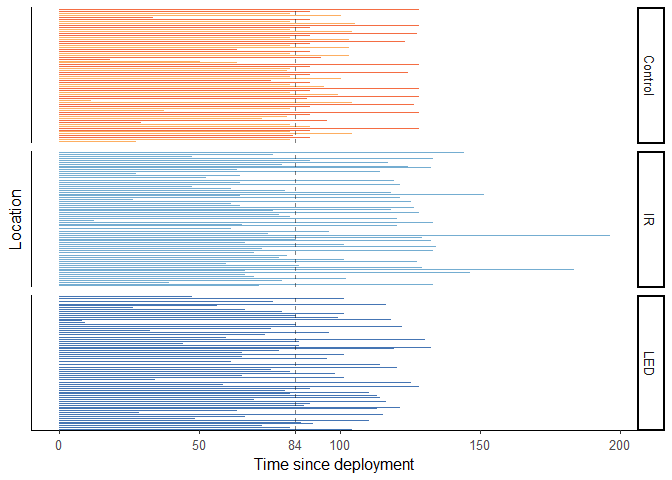
\includegraphics[scale=.8]{../R/glmm_sp_files/figure-html/period-length-wControl-1.png}
	\caption[Period lengths]%
	{Period lengths \par \small Vertical line represents the median IR period length, which was shorter than the median of the other groups. Data superceding the median were trimmed away for the GLMM  \label{fig:median_period}}
\end{figure}



\subsection{Equivalence test}
% Multiple testing i arkiv/method-ark
I used the standard significance level of $\alpha = .05$, and performed an equivalence test on my model outputs, using the function equivalence-test from the R package parameters ().%\cite{package-parameters}). %TODO

In an equivalence test, model parameters are tested against a Region of Practical Equivalence (ROPE) as opposed to merely one single mean value, thus accounting for the \emph{effect size} of each parameter.
If the parameters estimate and CI falls outside the ROPE, their null hypothesis is rejected. However, if the CI is inside the ROPE, H0 is accepted, no matter if a standard Null Hypothesis Significance Test (NHST) would have deemed it significant.

Inside the function equivalence-test I used the Two One-Sided Tests (TOST) rule, where the confidence interval (CI) is set to $1 - 2\times \alpha$. In my case that gave a narrow CI of 0.90.

For models from count data, the residual variance is often used to define the ROPE range. However, the description of the rope\_range function from the package bayestestR () states this threshold as "rather experimental" and that the range is probably often similar to the default [-0.1, 0.1] of a standardized parameter ($https://easystats.github.io/bayestestR/reference/rope_range.html$, accessed 11.3.2021). %TODO betre ref-metode for nettsider
Hence, I used the default ROPE range which corresponds to a negligible effect size according to Cohen, 1988.

%In the TOST procedure, the null hypothesis is the presence of a true effect of DL or DU, and the alternative hypothesis is an effect that falls within the equivalence bounds or the absence of an effect that is worthwhile to examine. \cite{Lakens2017}








%	\subsection*{Cox Proportional Hazards}
%%What I am in truth testing is each camera's chance of contracting a roe deer disease, or fox disease, and how that chance changes when "treated" with a white LED flash.
%
%
%However, the way I set up the GLMMs, it only takes into account whether a flash was present or not. It can't tell if the flash actually went off, or how many times it did.
%The time stamps from the white flash cameras were used to verify whether an animal was in fact flashed or not, which I then used as my main predictor in the modelling. 
%
%Therefore I set up a new column in my dataset, that told if the flash went off in synchrony with the IR camera or not (category yes/no).
%I then used the flashed-column to set up a time to event-analysis.
%Also called Survival analysis, time to event-analyses compares groups' risk of experiencing an event, and was first developed for use in medicinal studies, e.g. cancer risk studies (\cite{survival-book} ).
%
%The difference between the groups is called the hazard \emph{ratio}, and is \emph{assumed to be proportional} over time. That is, if after 2 days, the hazard of detecting a fox (i.e. experiencing an event) for the IR-group is twice as large compared to the white LED-group, it should remain twice as large after 25 days as well. Or in other words, the IR-group should detect twice as many foxes as the white LED-group in general.
%
%
%The Cox proportional hazards regression model (CPH model) (Cox, 1972), is a popular development of the time to event-analysis because it allows for more than one predictor. I used the R package Survival (\cite{survival-package}) and the function coxme from the R package coxme \cite{coxme-package} to perform a CPH with mixed effects (fixed and random effects). 
%Again, location ID and week of the year were used as random effects to account for differences between the camera sites and seasonal changes during the study period.
%
%
%As fixed effect I used the category for verified flash (yes/no).
%If a species was flashed, it went into the "flashed"-group, and time to next detection was recorded. 
%If the species didn't reappear it was "censored" from the model. Rather than saying that the species never reappeared (ie. time to event $= \infty$), the model assumes that had the study gone on longer there would eventually be an event. Conversely, in a cancer study, were death is the event, the survival of a patient during the study period wouldn't signify immortality, but rather that the study was ended too soon to record the event.
%
%
%In survival-analyses the time-variable is part of the outcome of the model. Event (i.e. detection) and time is joined as a Surv-object by the Surv function from the Survival package. 
%

%Both these models told me something about the fallacy of $H_0$, whether I could reject it, or fail to reject it.







%	\subsection*{P-tests and assumptions}

%For both the GLMM and the CPH mixed effect model, I used the Wald test as significance test, with xyz distribution over df degrees of freedom. osvosv. 


%Attention devoted to model assumptions! Viktig i Burton 2015
%The R package performance (cite) was used to check assumptions for GLMM, and ggeffects (cite) was used to visualize the results. 

%R package Survminer was used to visualize the results of the time to event analyses.
%The Schoenfeld test was used to check for the CPH's assumption of proportional hazards. 



%\subsection{AIC old}

%If you are using AIC model selection in your research, you can state this in your methods section. Report that you used AIC model selection, briefly explain the best-fit model you found, and state the AIC weight of the model.

%For each species, I used the Akaike Information Criterion (AIC) to select the best models excluding the flashed-predictor.
%Then, I added the flashed-predictor to each species top model, to see whether this effect could account for any remaining variation.
%
%
%Example: 
%
%We used AIC model selection to distinguish among a set of possible models describing the relationship between age, sex, sweetened beverage consumption, and body mass index.
%The best-fit model, carrying 97\% of the cumulative model weight, included every parameter with no interaction effects.

%After finding the best-fit model you can go ahead and run the model and evaluate the results. The output of your model evaluation can be reported in the results section of your paper.


